% !TeX spellcheck = cs_CZ
\begin{example}
  \textbf{Zemnicí elektroda}: Uvažujte zemnicí elektrodu ve tvaru koule o poloměru  
  $a=\SI{200}{\mm}$, uloženou do zeminy v hloubce, která je značně větší než je poloměr $a$. Pro 
  jednoduchost řešení dále předpokládejte, že přívodní drát je od zeminy izolován (obr.
  \ref{teo:fig022}). Zemina má měrnou vodivost $\gamma=\num[exponent-product =
  \cdot]{1,8e-2}\si{\per\ohm\per\m}$. Při zkratu teče přívodním drátem proud $I=\SI{50}{\A}$.
  Vypočítejte:

  {\centering
   \captionsetup{type=figure}
   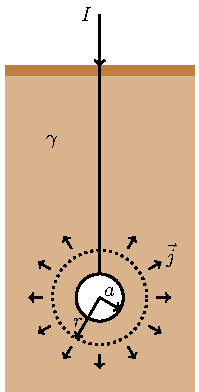
\includegraphics[width=0.5\linewidth]{teo_fig022.pdf}
   \captionof{figure}{Zemnicí elektroda
%   \cite[s.~263]{Musilova2009MA1}
   \label{teo:fig022}}
  \par}
  
  %----------------------------------
  % image: TEMP_zem_elektroda.tex label: \label{teo:fig022}
  % % \documentclass{article}
% \usepackage{tikz}
% \usetikzlibrary{decorations.markings}
% \usetikzlibrary{intersections}
% \usetikzlibrary{calc}

% \begin{document}
   {\centering  
    \begin{tikzpicture}[scale=0.8, every node/.style={scale=1}]
      \coordinate (pCenter) at (0,-5);
      \fill[brown!60] (-2,-0.2) rectangle (2,-7);
      \draw[color=brown, line width=5pt] (-2,-0.2) -- +(4,0); 
      \draw[->,line width=1pt] (0,1) node[left] {$I$} -- (0,-0.1);        
      \draw[line width=1pt] (0,0) -- (pCenter);
      \draw[line width=1pt,color=black, fill=white]
           (pCenter) circle[radius=0.5];
      \draw[line width=1pt, dotted]
           (pCenter) circle[radius=1];
      \foreach \angle in
          {0, 30, 60, 120, 150, 180, 210, 240, 270, 300, 330}
      {
        \draw[->, line width=0.75pt] (pCenter)++(\angle:1.2) -- +(\angle:0.3);        
      }
      \draw[<->, thick] (pCenter)++(240:1) coordinate(pR) -- (pCenter) -- +(330:0.5) coordinate(pA); 
      \node[above] at ($ (pCenter)!0.5!(pA) $) {$a$};     
      \node[above] at ($ (pCenter)!0.9!(pR) $) {$r$}; 
      \node[above] at (-1,-2) {$\gamma$};
      \node[above] at (+1.5,-4.5) {$\vec{j}$};
    \end{tikzpicture}
    \captionsetup{type=figure}
    \captionof{figure}{Zemnicí elektroda}
    \label{TEMP:fig_zem_elektroda}
  \par}
  
% \end{document}    
  %----------------------------------         
  \begin{enumerate}[label=\emph{\alph*})]
    \item Závislost potenciálu $\varphi=\varphi(r)$ elektrického pole, které se vytvoří v
          zemině při zkratu, kde $r$ je vzdálenost od středu elektrody. Potenciál normujte
          volbou $\varphi(\infty)=0$.
    \item Zemnicí odpor elektrody, který je definován vztahem $$R_z=\frac{U_z}{I_z},$$ kde
          $U_z = \varphi(a)-\varphi(b)$ je zemnicí napětí 
    \item Ztrátový výkon při zkratu.
  \end{enumerate}
  Řešení:    
  Ekvipotenciální a proudové plochy mají zřejmě kulový tvar se středem totožným s geometrickým 
  středem elektrody. Proudová hustota na kulové ploše obecného poloměru $r$ (viz. obr. 
  \ref{teo:fig022}) je $$\vec{j}=\frac{I}{4\pi r^2}\vec{n},$$ kde $\vec{n}$ je 
  jednotkový vektor ve směru normály. Pak v bodech na této ploše musí být elektrické pole o 
  intenzitě $\vec{E}$, kterou určíme ze vztahu
  \begin{equation*}
    \vec{j}= \gamma\vec{E}\rightarrow\vec{E}=
    \frac{\vec{j}}{\gamma}=\frac{I}{4\pi\gamma r^2}\vec{n}.
  \end{equation*}
  Závislost potenciálu $\varphi=\varphi(r)$ tohoto elektrického pole stanovíme pomocí následujícího 
  integrálu
  \begin{equation}
    \varphi = - \int\vec{E}d\vec{r}+C = -\frac{I}{4\pi\gamma}\int\frac{dr}{r^2} + C 
            =   \frac{I}{4\pi\gamma r} + C, \nonumber
  \end{equation} 
  kde integrační konstantu $C$ určíme z okrajové podmínky $\varphi(\infty)=0$, odkud $C=0$.
  Hledaná závislost potenciálu je
  \begin{equation*}
    \varphi = \frac{I}{4\pi\gamma r}, \qquad r\in\langle a, \infty). 
  \end{equation*}           
  
  Zemina, v níž je uložena elektroda, je vlastně rezistorem, jehož jeden okraj tvoří elektrodu
  a druhým okrajem je nekonečně rozlehlý vodivý prostor. Potenciální rozdíl mezi těmito okraji je
  \begin{equation*}
    U_z = \varphi(a) - \varphi(\infty)= \frac{I}{4\pi\gamma a},
  \end{equation*} 
  \begin{minipage}[t]{0.5\textwidth}% first column            
    odkud zemnicí odpor 
    \begin{equation*}
      R_z = \frac{U_z}{I} = \frac{1}{4\pi\gamma a} = \SI{22,1}{\ohm}
    \end{equation*}
  \end{minipage}
  \begin{minipage}[t]{0.5\textwidth}% second column    
    a ztrátový výkon 
    \begin{equation*}
      P_z = R_z\cdot I^2 = \SI{55,3}{\kilo\watt}. 
    \end{equation*}
  \end{minipage}
\end{example}


